% MH1812 — Chapter 2: Sets (0->100 ground-up)
\chapter[Sets]{Sets, Power Sets, Venn Diagrams and Relations}
\label{ch:sets}

\begin{quote}
\emph{``A set is a Many that allows itself to be thought of as a One.''} --- Georg Cantor. Databases, types, and state spaces are all sets.
\end{quote}

\noindent\fbox{\parbox{\dimexpr\linewidth-2\fboxsep-2\fboxrule}{%
\textbf{From zero: sets from dots.} Picture a bag of dots; a set is just which dots are in the bag. We formalise membership, build operations (union, intersection, complement), count subsets (power set), draw Venn regions, and then generalise to relations as sets of pairs.}}
\vspace{0.4em}

\section*{Learning Outcomes}
After this chapter you will be able to:
\begin{enumerate}[label=(L\arabic*)]
    \item use set notation ($\in,\subseteq,\subsetneq,|S|,\emptyset,\mathcal{P}(S),A\times B$) fluently;
    \item compute unions, intersections, complements, differences and power sets;
    \item count subsets and interpret $|\mathcal{P}(S)|=2^{|S|}$;
    \item read and shade Venn diagrams for arbitrary set expressions;
    \item define relations, their properties, closures, and equivalence/partial orders.
\end{enumerate}

% ============================================================
\section{Sets and Membership}
\label{sec:sets-membership}
A \emph{set} is an unordered collection of distinct objects. $x\in S$ means $x$ is a member; $x\notin S$ otherwise. $S\subseteq T$ if every $x\in S$ also $x\in T$. $S=T$ iff $S\subseteq T$ and $T\subseteq S$. $S\subsetneq T$ if $S\subseteq T$ and $S\neq T$. $\emptyset$ has no members; $|\emptyset|=0$. Universe $U$ is the ambient set for complements.

Common universes: $\mathbb{N}=\{0,1,2,\dots\}$, $\mathbb{Z}$, $\mathbb{Q}$, $\mathbb{R}$, $\mathbb{Z}^+$, $[n]=\{1,\dots,n\}$. Interval $[a,b]$, $(a,b)$ have usual meaning over $\mathbb{R}$.

Operations (picture as Venn shading):
\begin{align*}
A\cup B &=\{x: x\in A\lor x\in B\},\\
A\cap B &=\{x: x\in A\land x\in B\},\\
A\setminus B &=\{x: x\in A\land x\notin B\},\quad \bar A =U\setminus A,\\
A\oplus B &=(A\setminus B)\cup(B\setminus A)\quad\text{(symmetric difference).}
\end{align*}

Laws mirror logic: De Morgan $\overline{A\cup B}=\bar A\cap\bar B$, distributivity, etc., because $x\in A\cup B\equiv x\in A\lor x\in B$.

\begin{figure}[h]\centering
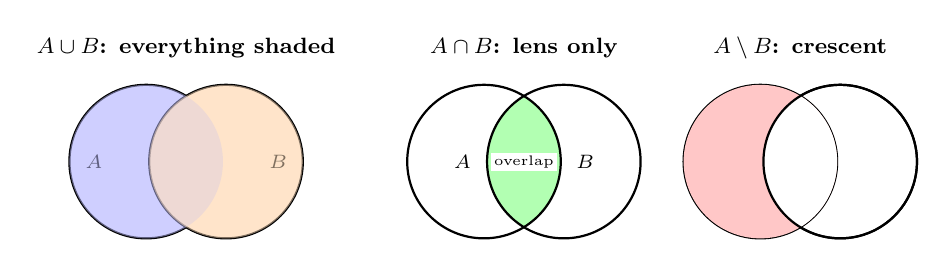
\begin{tikzpicture}[scale=0.78,every node/.style={font=\scriptsize}]
% Venn two sets with shading for union vs intersection
\begin{scope}
\draw[thick,fill=blue!12] (0,0) circle (1.25);
\draw[thick,fill=orange!16] (1.3,0) circle (1.25);
\node at (-0.85,0) {$A$}; \node at (2.15,0) {$B$};
\node[font=\footnotesize\bfseries] at (0.65,1.85) {$A\cup B$: everything shaded};
\fill[blue!25,opacity=0.5] (0,0) circle (1.25);
\fill[orange!25,opacity=0.5] (1.3,0) circle (1.25);
\end{scope}
\begin{scope}[xshift=5.5cm]
\begin{scope}
\clip (0,0) circle (1.25);
\fill[green!30] (1.3,0) circle (1.25);
\end{scope}
\draw[thick] (0,0) circle (1.25);
\draw[thick] (1.3,0) circle (1.25);
\node at (-0.35,0) {$A$}; \node at (1.65,0) {$B$};
\node[font=\footnotesize\bfseries] at (0.65,1.85) {$A\cap B$: lens only};
\node[font=\tiny,fill=white,inner sep=1pt] at (0.65,0) {overlap};
\end{scope}
\begin{scope}[xshift=10cm]
\draw[thick] (0,0) circle (1.25);
\draw[thick] (1.3,0) circle (1.25);
\fill[red!22] (0,0) circle (1.25);
\begin{scope}
\clip (0,0) circle (1.25);
\fill[white] (1.3,0) circle (1.25);
\end{scope}
\draw[thick] (1.3,0) circle (1.25);
\node[font=\footnotesize\bfseries] at (0.65,1.85) {$A\setminus B$: crescent};
\end{scope}
\end{tikzpicture}
\caption{Three Venn shadings that translate directly to $\lor$, $\land$, $\land\neg$. Colour = membership.}
\label{fig:venn-basic}
\end{figure}

\begin{example}[Set laws by element argument]
$A\cap(B\cup C)=(A\cap B)\cup(A\cap C)$. Proof: $x\in$ LHS $\iff x\in A\land(x\in B\lor x\in C)\iff(x\in A\land x\in B)\lor(x\in A\land x\in C)\iff x\in$ RHS.
\end{example}

\section{Power Sets and Cartesian Products}
\label{sec:powerset}
The \emph{power set} $\mathcal{P}(S)=\{T:T\subseteq S\}$ collects all subsets. If $S=\{a,b,c\}$ then $\mathcal{P}(S)$ has $2^3=8$ members: $\emptyset,\{a\},\{b\},\{c\},\{a,b\},\{a,c\},\{b,c\},\{a,b,c\}$.

\begin{theorem}[$|\mathcal{P}(S)|=2^{|S|}$]
For finite $S$ with $|S|=n$, $|\mathcal{P}(S)|=2^n$. Each subset corresponds to an $n$-bit string (choose in/out per element); $2$ choices per position $\Rightarrow 2^n$ strings.
\end{theorem}

\begin{figure}[h]\centering
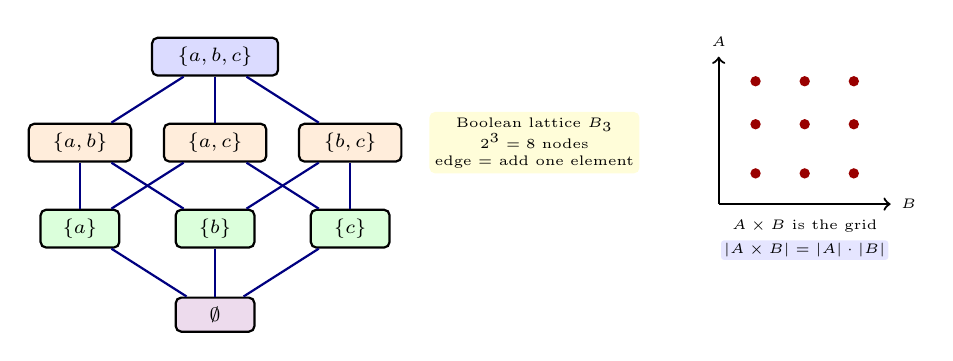
\begin{tikzpicture}[scale=0.78,every node/.style={font=\scriptsize}]
% Boolean lattice for n=3
\node[draw,thick,rounded corners=2pt,fill=blue!14,minimum width=1.6cm] (top) at (0,3.2) {$\{a,b,c\}$};
\node[draw,thick,rounded corners=2pt,fill=orange!14,minimum width=1.3cm] (ab) at (-2.2,1.8) {$\{a,b\}$};
\node[draw,thick,rounded corners=2pt,fill=orange!14,minimum width=1.3cm] (ac) at (0,1.8) {$\{a,c\}$};
\node[draw,thick,rounded corners=2pt,fill=orange!14,minimum width=1.3cm] (bc) at (2.2,1.8) {$\{b,c\}$};
\node[draw,thick,rounded corners=2pt,fill=green!14,minimum width=1.0cm] (a) at (-2.2,0.4) {$\{a\}$};
\node[draw,thick,rounded corners=2pt,fill=green!14,minimum width=1.0cm] (b) at (0,0.4) {$\{b\}$};
\node[draw,thick,rounded corners=2pt,fill=green!14,minimum width=1.0cm] (c) at (2.2,0.4) {$\{c\}$};
\node[draw,thick,rounded corners=2pt,fill=violet!14,minimum width=1.0cm] (bot) at (0,-1.0) {$\emptyset$};
\foreach \u/\v in {top/ab,top/ac,top/bc,ab/a,ab/b,ac/a,ac/c,bc/b,bc/c,a/bot,b/bot,c/bot}
  \draw[thick,blue!50!black] (\u)--(\v);
\node[font=\tiny,fill=yellow!15,rounded corners=2pt,inner sep=2pt,align=center] at (5.2,1.8) {Boolean lattice $B_3$\\$2^3=8$ nodes\\edge $=$ add one element};
% Cartesian product picture on right
\begin{scope}[xshift=8.2cm,yshift=0.8cm]
\draw[->,thick] (0,0)--(2.8,0) node[right,font=\tiny] {$B$};
\draw[->,thick] (0,0)--(0,2.4) node[above,font=\tiny] {$A$};
\foreach \x in {0.6,1.4,2.2} \foreach \y in {0.5,1.3,2.0} \fill[red!60!black] (\x,\y) circle (2.4pt);
\node[font=\tiny] at (1.4,-0.35) {$A\times B$ is the grid};
\node[font=\tiny,fill=blue!10,rounded corners=1pt,inner sep=1pt] at (1.4,-0.75) {$|A\times B|=|A|\cdot|B|$};
\end{scope}
\end{tikzpicture}
\caption{Left: power set as Boolean lattice (Hasse diagram). Right: Cartesian product as grid of ordered pairs.}
\label{fig:powerset-cartesian}
\end{figure}

The \emph{Cartesian product} $A\times B=\{(a,b):a\in A,b\in B\}$ has $|A\times B|=|A|\cdot|B|$ (product rule, Ch.~5). $A\times B\neq B\times A$ generally; order matters.

\begin{lstlisting}[language=Python]
# Power set via bit masks -- matches |P(S)| = 2^n
def powerset(s):
    s = list(s)
    n = len(s)
    return [{s[j] for j in range(n) if (mask>>j)&1} for mask in range(1<<n)]
print(powerset({'a','b','c'}))
\end{lstlisting}

\section{Relations}
\label{sec:relations}
A \emph{relation} $R$ from $A$ to $B$ is any $R\subseteq A\times B$. Write $a\,R\,b$ for $(a,b)\in R$. On a single set $A$, $R\subseteq A\times A$ is a relation on $A$.

\begin{figure}[h]\centering
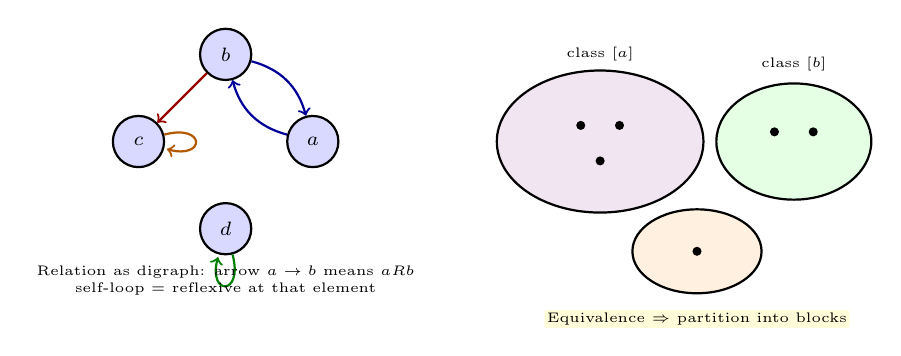
\begin{tikzpicture}[scale=0.82,every node/.style={font=\scriptsize}]
% Digraph of relation
\foreach \i/\name in {0/a,1/b,2/c,3/d} {\node[draw,circle,thick,fill=blue!15,minimum size=0.65cm] (n\i) at (90*\i:1.35) {$\name$};}
\draw[->,thick,blue!60!black] (n0) edge[bend left] (n1);
\draw[->,thick,blue!60!black] (n1) edge[bend left] (n0);
\draw[->,thick,red!60!black] (n1) -- (n2);
\draw[->,thick,orange!70!black] (n2) edge[loop right] (n2);
\draw[->,thick,green!50!black] (n3) edge[loop below] (n3);
\node[font=\tiny,align=center] at (0,-2.15) {Relation as digraph: arrow $a\to b$ means $aRb$\\self-loop $=$ reflexive at that element};
% Equivalence classes partition
\begin{scope}[xshift=5.8cm]
\draw[thick,fill=violet!10,rounded corners=4pt] (0,0) ellipse (1.6 and 1.1);
\draw[thick,fill=green!10,rounded corners=4pt] (3.0,0) ellipse (1.2 and 0.9);
\draw[thick,fill=orange!12,rounded corners=4pt] (1.5,-1.7) ellipse (1.0 and 0.65);
\foreach \x/\y in {-0.3/0.25,0.3/0.25,0/-0.3} \fill ( \x,\y) circle (2pt);
\foreach \x/\y in {2.7/0.15,3.3/0.15} \fill (\x,\y) circle (2pt);
\fill (1.5,-1.7) circle (2pt);
\node[font=\tiny] at (0,1.35) {class $[a]$};
\node[font=\tiny] at (3.0,1.2) {class $[b]$};
\node[font=\tiny,fill=yellow!15,rounded corners=1pt,inner sep=1pt] at (1.5,-2.75) {Equivalence $\Rightarrow$ partition into blocks};
\end{scope}
\end{tikzpicture}
\caption{Left: digraph of a relation. Right: equivalence relation partitions the set into disjoint blocks.}
\label{fig:relation-digraph}
\end{figure}

Properties for $R$ on $A$: \emph{reflexive} ($\forall a\,aRa$), \emph{symmetric} ($aRb\Rightarrow bRa$), \emph{antisymmetric} ($aRb\land bRa\Rightarrow a=b$), \emph{transitive} ($aRb\land bRc\Rightarrow aRc$).

\begin{definition}[Equivalences and orders]
$R$ is an \emph{equivalence} if reflexive, symmetric, transitive --- it partitions $A$ into \emph{equivalence classes} $[a]=\{b:aRb\}$. $R$ is a \emph{partial order} if reflexive, antisymmetric, transitive; a \emph{total order} if additionally comparable.
\end{definition}


\begin{lstlisting}[language=Python]
# Sets in Python directly mirror the maths
A = {1,2,3,4}; B = {3,4,5}
print(A | B, A & B, A - B, A ^ B)  # union, inter, diff, sym diff
# Relation as set of pairs; check reflexivity
def is_reflexive(R, A): return all((a,a) in R for a in A)
R = {(1,1),(2,2),(3,3),(1,2),(2,1)}
print(is_reflexive(R, {1,2,3}))
\end{lstlisting}

\begin{example}
``$=$'' and ``same birthday'' are equivalences; ``$\le$'' on $\mathbb{Z}$ and ``$\subseteq$'' on $\mathcal{P}(S)$ are partial orders (the latter not total for $|S|\ge2$).
\end{example}

Closures: reflexive/symmetric/transitive closures add minimal pairs to achieve the property; transitive closure $R^*$ is reachability in the digraph (Floyd--Warshall / BFS).


\begin{remark}[Why $\emptyset\subseteq S$ always]
$\emptyset\subseteq S$ vacuously: ``$\forall x(x\in\emptyset\to x\in S)$'' has false antecedent for every $x$, so the implication is true on every row. Similarly $S\subseteq S$.
\end{remark}

\begin{theorem}[Inclusion--Exclusion for two sets]
$|A\cup B|=|A|+|B|-|A\cap B|$. Venn lens is counted twice, subtract once.
\end{theorem}
\begin{proof} Count $x\in A\cup B$: if $x$ in exactly one, contributes $1$; if in both, $1+1-1=1$.
\end{proof}


\begin{example}[Set builder pitfalls]
$\{x\in\mathbb{Z}:x^2<5\}=\{-2,-1,0,1,2\}$. Always state the universe; $\{x:x^2<5\}$ over $\mathbb{R}$ is $(-\sqrt5,\sqrt5)$.
\end{example}

\begin{theorem}[Distributivity]
$A\cap(B\cup C)=(A\cap B)\cup(A\cap C)$ and dually $A\cup(B\cap C)=(A\cup B)\cap(A\cup C)$.
\end{theorem}

\begin{remark}[Russell's paradox sketch]
The ``set of all sets not containing themselves'' cannot exist consistently --- reason ZFC restricts comprehension. Not needed for finite CS sets, but warns against naive ``set of all sets''.
\end{remark}

Venn diagrams are not proofs, but they are excellent for conjecturing set identities before proving them algebraically.
The empty set is a subset of every set, vacuously, which often serves as the base case of set inductions.
Power sets grow exponentially: adding one element doubles the number of subsets.
Bit-strings and subsets are the same idea in different costumes, linked by characteristic functions.
Cartesian products model tables in relational databases: each row is an ordered pair.
A relation can be stored as a Boolean matrix or an adjacency list, mirroring its digraph view.
Equivalence classes partition a set like countries partition the globe, disjoint and covering.
Partial orders model dependencies: $a\le b$ means $a$ must come before $b$.
Closures add the minimal edges needed, like adding the missing transitive flights to connect all reachable cities.
Inclusion--exclusion corrects overcounting, essential for counting unions without double-counting overlaps.
Venn diagrams are not proofs, but they are excellent for conjecturing set identities before proving them algebraically.
The empty set is a subset of every set, vacuously, which often serves as the base case of set inductions.
Power sets grow exponentially: adding one element doubles the number of subsets.
Bit-strings and subsets are the same idea in different costumes, linked by characteristic functions.
Cartesian products model tables in relational databases: each row is an ordered pair.
A relation can be stored as a Boolean matrix or an adjacency list, mirroring its digraph view.
Equivalence classes partition a set like countries partition the globe, disjoint and covering.
Partial orders model dependencies: $a\le b$ means $a$ must come before $b$.
Closures add the minimal edges needed, like adding the missing transitive flights to connect all reachable cities.
Inclusion--exclusion corrects overcounting, essential for counting unions without double-counting overlaps.
Venn diagrams are not proofs, but they are excellent for conjecturing set identities before proving them algebraically.
The empty set is a subset of every set, vacuously, which often serves as the base case of set inductions.
Power sets grow exponentially: adding one element doubles the number of subsets.
Bit-strings and subsets are the same idea in different costumes, linked by characteristic functions.
Cartesian products model tables in relational databases: each row is an ordered pair.
A relation can be stored as a Boolean matrix or an adjacency list, mirroring its digraph view.
Equivalence classes partition a set like countries partition the globe, disjoint and covering.
Partial orders model dependencies: $a\le b$ means $a$ must come before $b$.
Closures add the minimal edges needed, like adding the missing transitive flights to connect all reachable cities.
Inclusion--exclusion corrects overcounting, essential for counting unions without double-counting overlaps.
Venn diagrams are not proofs, but they are excellent for conjecturing set identities before proving them algebraically.
The empty set is a subset of every set, vacuously, which often serves as the base case of set inductions.

\section{Worked Example: Counting with Sets}
How many NTU students take MH1812 or SC2001? Let $A=$ MH1812 cohort, $B=$ SC2001 cohort. Inclusion--exclusion gives $|A\cup B|=|A|+|B|-|A\cap B|$. If $|A|=300$, $|B|=250$, $|A\cap B|=80$, then $|A\cup B|=470$. Without subtracting the overlap we double-count.

Power set example: a $3$-bit binary string $b_2b_1b_0$ encodes a subset of $\{a,b,c\}$: $b_i=1$ means include element $i$. Thus $101$ encodes $\{a,c\}$. This bijection between $\{0,1\}^3$ and $\mathcal{P}(S)$ proves $|\mathcal{P}(S)|=2^3$ and generalises to $2^n$; it is also how a computer stores a subset as a bitmask.

Relation closure example: $R=\{(1,2)\}$ on $\{1,2,3\}$ is not transitive, not symmetric. Its transitive closure adds nothing beyond $R$ (no chain of length $2$), but symmetric closure adds $(2,1)$, and reflexive closure adds $(1,1),(2,2),(3,3)$.

% ============================================================
\section{Chapter Notes}
Cantor created set theory (1870s); Russell's paradox forced axiomatisation (ZFC). Power sets link to bit-strings and to complexity ($2^n$ subsets). Venn diagrams (John Venn, 1880) remain a debugging tool for SQL and Boolean logic.

% ============================================================
\section{Exercises}
\label{sec:ch02-exercises}
\begin{enumerate}[label=E2.\arabic*, leftmargin=*, itemsep=0.6em]
\item \textbf{Operations.} Let $A=\{1,2,3,4\}$, $B=\{3,4,5\}$. Compute $A\cup B$, $A\cap B$, $A\setminus B$, $\bar A$ with $U=[1..6]$, $A\oplus B$, $A\times B$, and $|\mathcal{P}(A)|$.
\item \textbf{Venn shading.} Shade (a) $(A\cap\bar B)\cup(B\cap\bar A)$ (which equals $A\oplus B$), (b) $\overline{A\cup B}\cup(A\cap B)$. Verify De Morgan $\overline{A\cap B}=\bar A\cup\bar B$ by shading both sides.
\item \textbf{Power set proof.} Prove by induction or binomial sum that $\sum_{k=0}^{n}\binom{n}{k}=2^n$ counts subsets by size. List $\mathcal{P}(\{1,2,3,4\})$ grouped by cardinality $k$.
\item \textbf{Relations.} On $A=\{1,2,3\}$ let $R=\{(1,1),(2,2),(3,3),(1,2),(2,1)\}$. Check each property and decide if $R$ is equivalence or partial order. Find its equivalence classes or explain failure.
\item \textbf{Closures.} For $R=\{(1,2),(2,3)\}$ on $\{1,2,3,4\}$ find reflexive, symmetric, and transitive closures. Draw digraphs before and after closure.
\end{enumerate}
% End of Chapter 2
